\section{Results}

\subsection{Visualisation}

We were able to develop command-line programs to show both the kernelization
and branching algorithms working in real-time. Obviously, the speed of the
algorithms have been slowed to allow for the user to understand what's
happening at each step. Both programs take a path to an edge list file and a
\(k\) value as command-line arguments so visualisations can be produced of
different graphs at different \(k\) values. This gives the ability to see how a
kernel of a graph changes depending on the value of \(k\).

Naturally, there is a limit to the size of the graph being displayed. On top of
having the entire graph in memory and the memory required for running each
algorithm, memory is also needed for rendering the image for each frame.

\begin{figure}[htb]
    \centering
    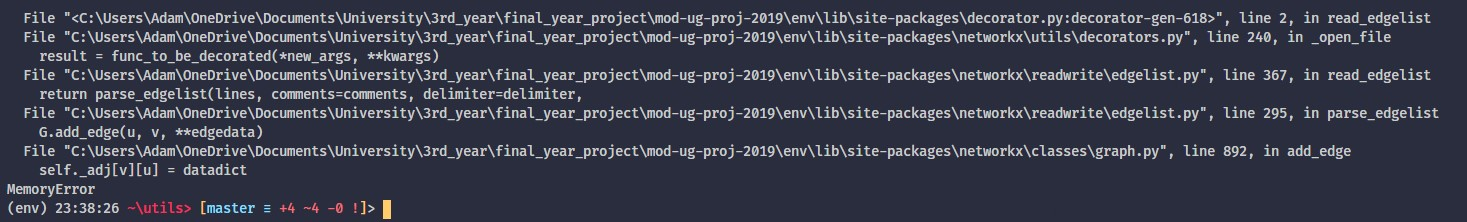
\includegraphics[width=\textwidth]{memory-error.jpg}
    \caption{Memory error}
\end{figure}

\subsubsection{Kernelization}

Being the visually more interesting and intricate algorithm, it made sense for
us to focus our effort on the kernelization algorithm. In Figure
\ref{fig:kernelization_visualisation}, you can see that we have split the plot
into two. On the left side we show the entire graph, marking which vertices and
edges have been added to the kernel as well as which edge of the graph is
currently being processed. A subtitle shows counts of the number of nodes and
edges in the graph. On the right we show the kernel being built up as the
algorithm progresses. All vertices and edges of the kernel exist in the same
position as they do in the graph so it is easy to see how the kernel resembles
the core components of the whole graph once enough vertices have been added to
the kernel. Red mark those vertices and edges that are part of the maximal
matching the kernelization algorithm maintains. Black marks the neighbours of
each matched vertex. A subtitle also shows information relating to the kernel
at each step as well as how the kernel relates to the graph in terms of its
size.

\begin{figure}[htb]
    \centering
    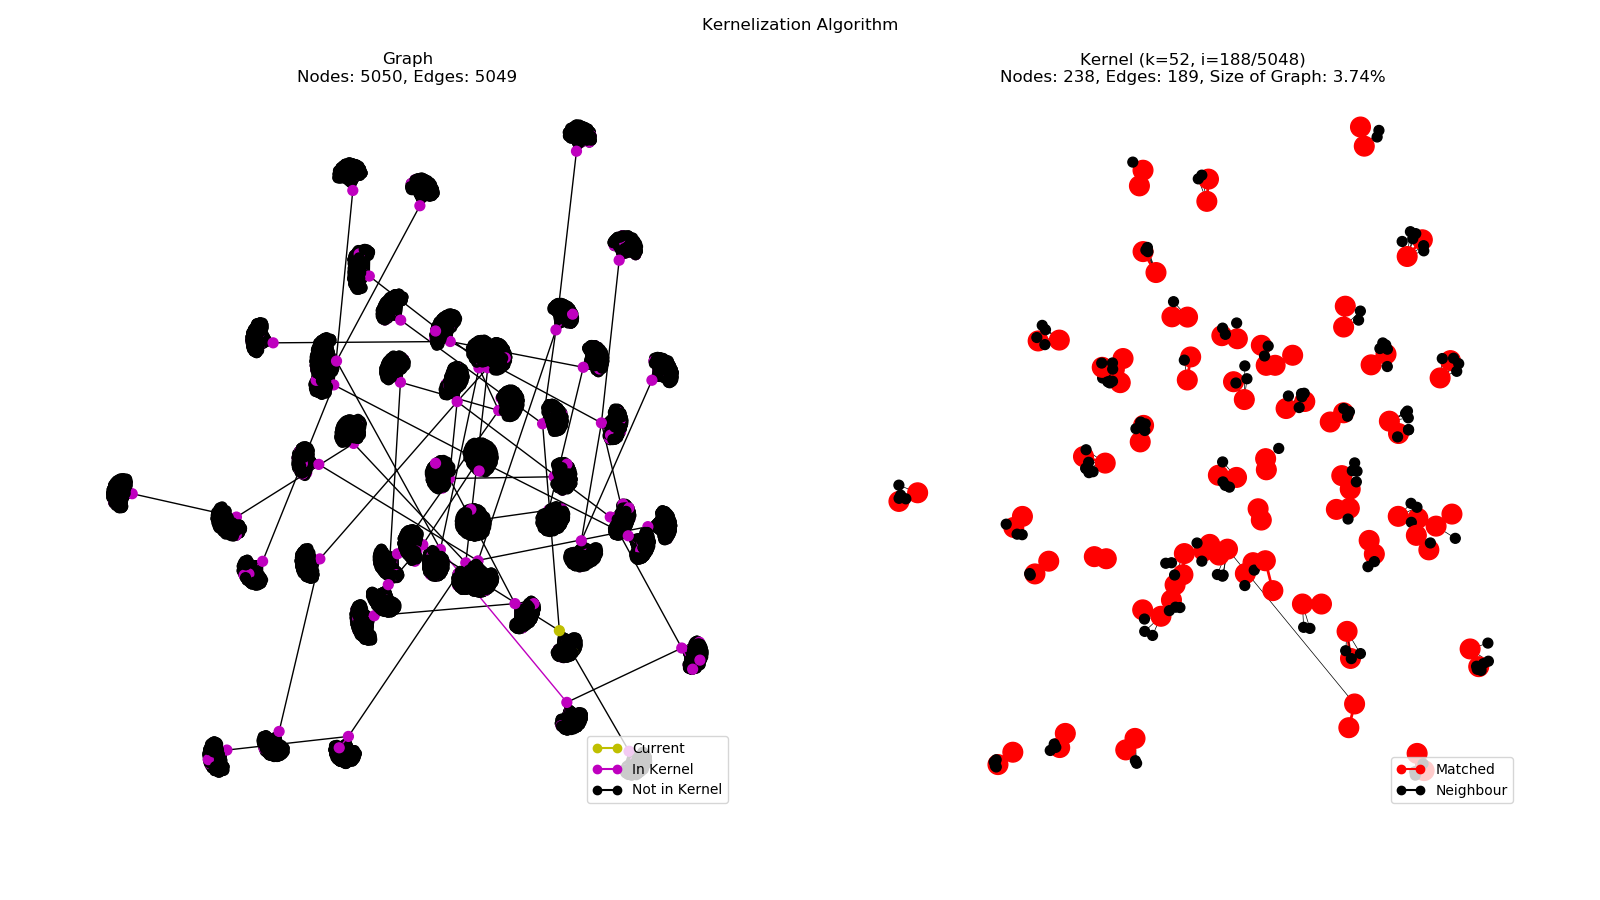
\includegraphics[width=\textwidth]{visuals_kernelization.png}
    \caption{Streaming Kernelization Visualisation}
    \label{fig:kernelization_visualisation}
\end{figure}

bit about graph drawing?

While the method we chose in Matplotlib for creating live demonstrations was
rather crude, Matplotlib does include classes to create animations with that
are able to then be exported into video formats. Using this, we ported over the
code used to generate the live demonstration into a new program that creates
videos exported to whichever format is specified. This allows for easy sharing
of GIFs showing the kernelization in practice.

\subsubsection{Branching}

The branching algorithm is much simpler visually. We created a live
demonstration that shows the search tree and the depth-first search being
applied to it. The yellow vertex marks the current vertex cover configuration
being tested and a boldened trail of edges shows the current path being taken.
The binary string being used for the path is shown towards the top left as well
as an underscore under the current binary value. Below that is the current edge
of the stream. A subtitle shows the current depth and edge index.

\begin{figure}[htb]
    \centering
    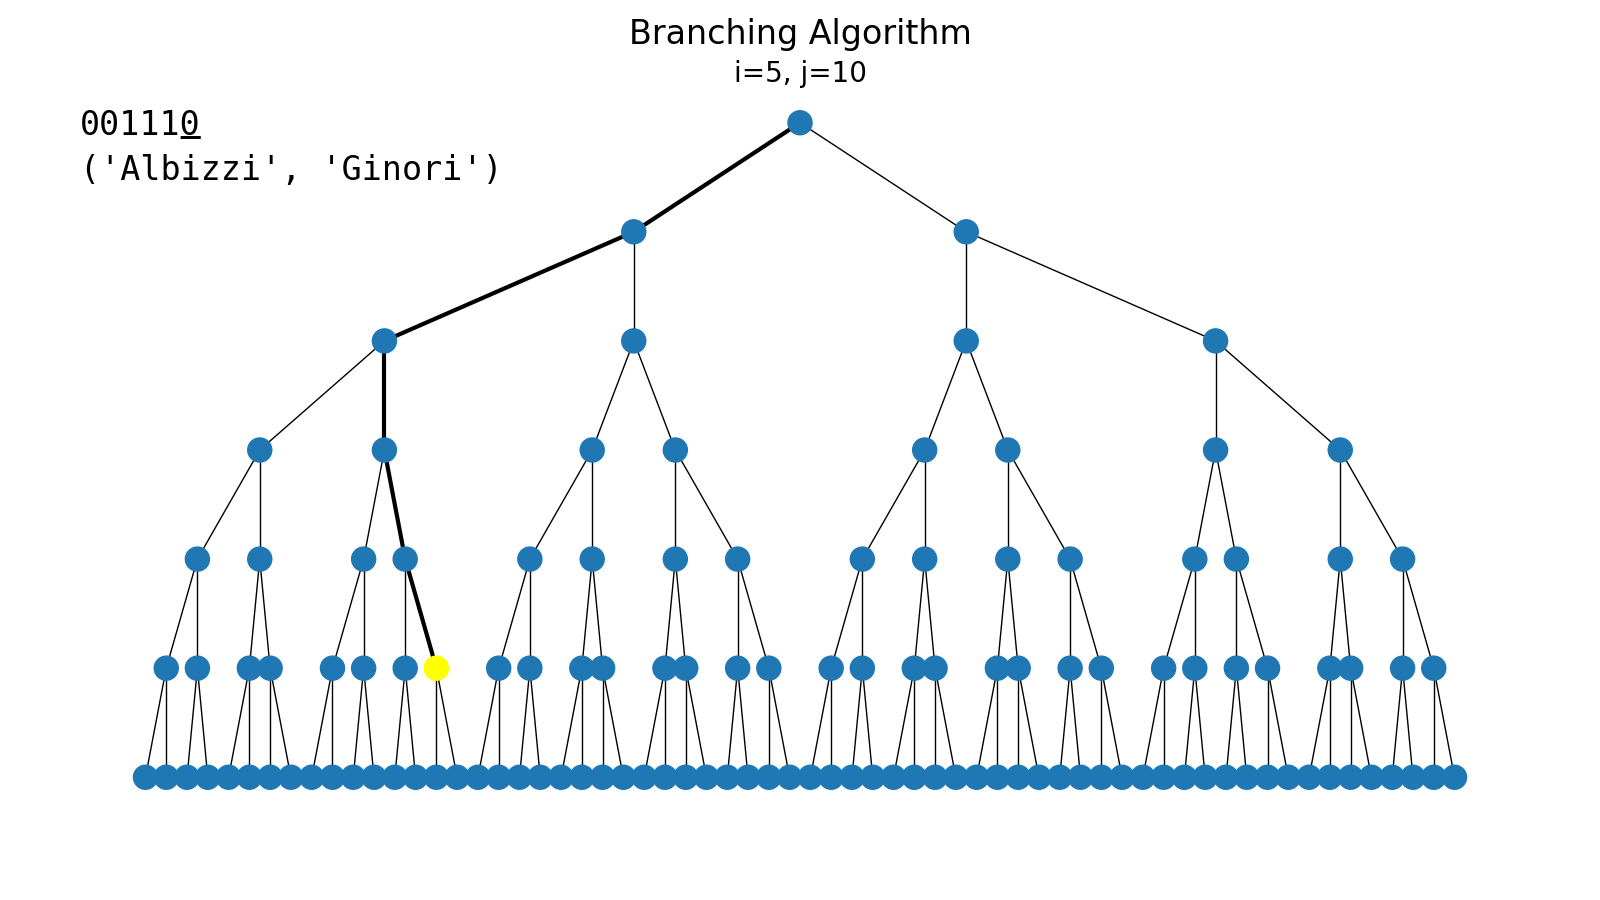
\includegraphics[width=\textwidth]{visuals_branching.png}
    \caption{Streaming Branching Visualisation}
    \label{fig:branching_visualisation}
\end{figure}

It should be noted that, due to the exponential nature of trees, a \(k\) value
of 10 or more will take significantly longer to load. So, it is advised to use
only the visualisation for \(k\) values smaller than this. From the Figure
\ref{fig:branching_visualisation} you can see that already at \(k=6\), the
bottom line of vertices is getting cramped for space.

\subsection{Performance Benchmarking}

\subsubsection{Memory Profiling}

Nothing here surprised us but it's always nice to be able to see the truth laid
out in front of you.

\paragraph{Kernelization}

\begin{figure}[H]
    \centering
    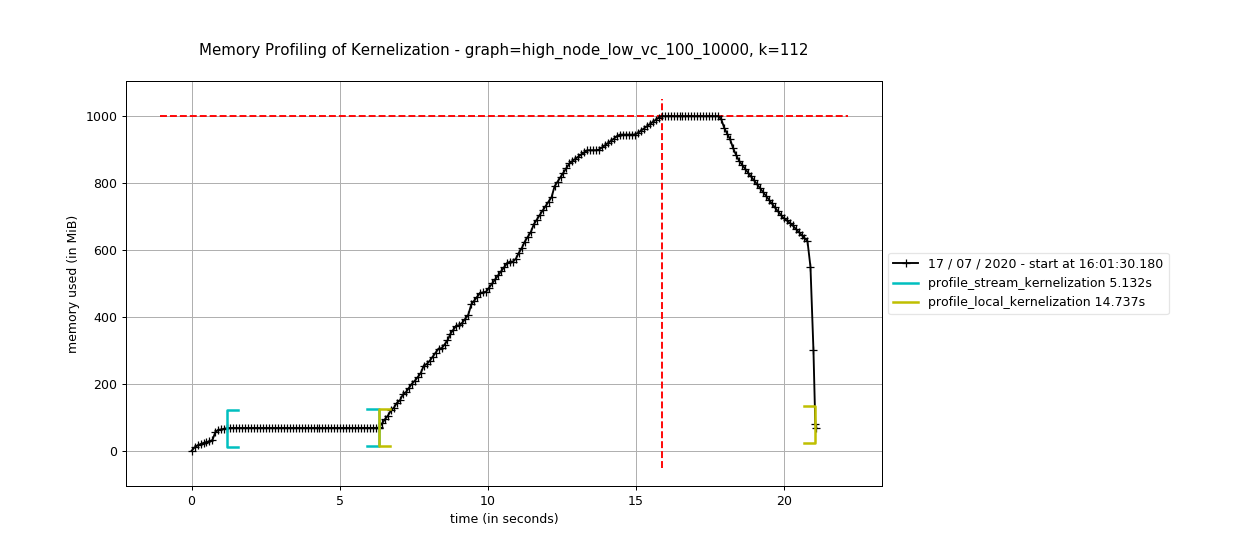
\includegraphics[width=\textwidth]{benchmark_memory_kernelization_100_10000.png}
    \caption{Memory Profiling of Kernelization}
    \label{fig:benchmark_mem_kernelization}
\end{figure}

\paragraph{Branching}

\begin{figure}[H]
    \centering
    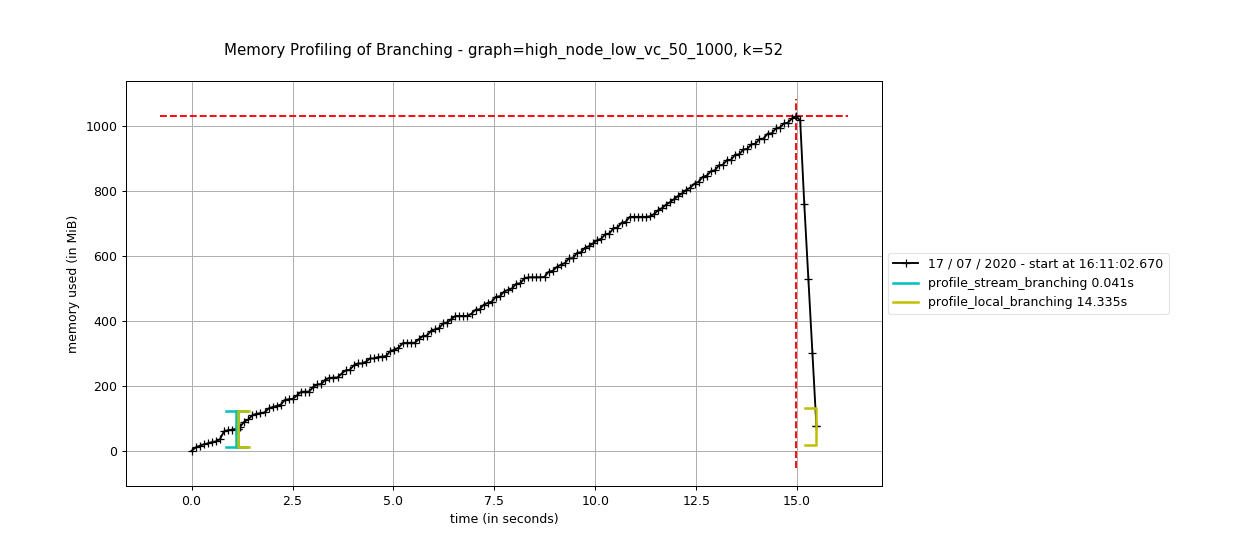
\includegraphics[width=\textwidth]{benchmark_memory_branching_50_1000.png}
    \caption{Memory Profiling of Branching}
    \label{fig:benchmark_mem_branching}
\end{figure}

\subsubsection{Runtime Analysis}

\paragraph{Kernelization}

\begin{figure}[H]
    \centering
    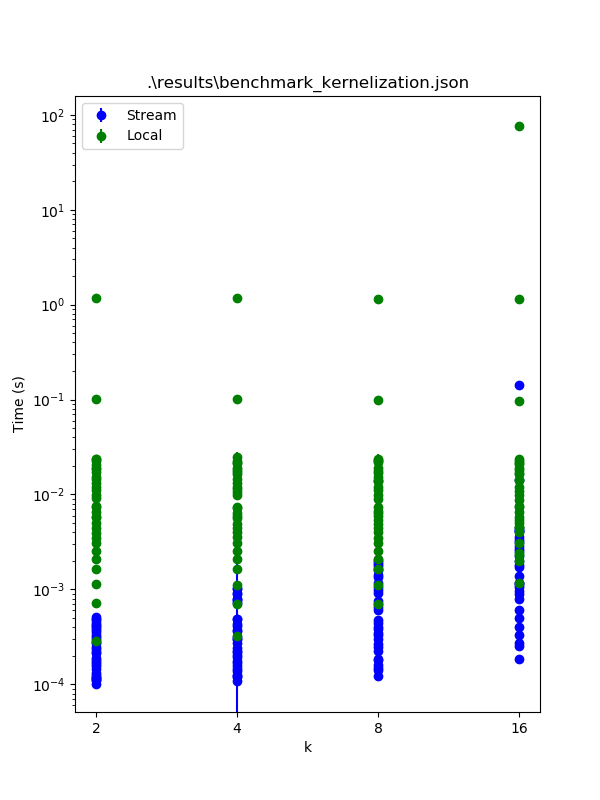
\includegraphics[width=\textwidth]{benchmark_time_kernelization.png}
    \caption{Runtimes of Kernelization}
    \label{fig:benchmark_time_kernelization}
\end{figure}

\paragraph{Branching}

Due to the branching algorithm having a runtime of \(O(2^k)\), it quickly
became clear that we weren't going to be able to gather as much data as we had
initially wanted.

\begin{figure}[H]
    \centering
    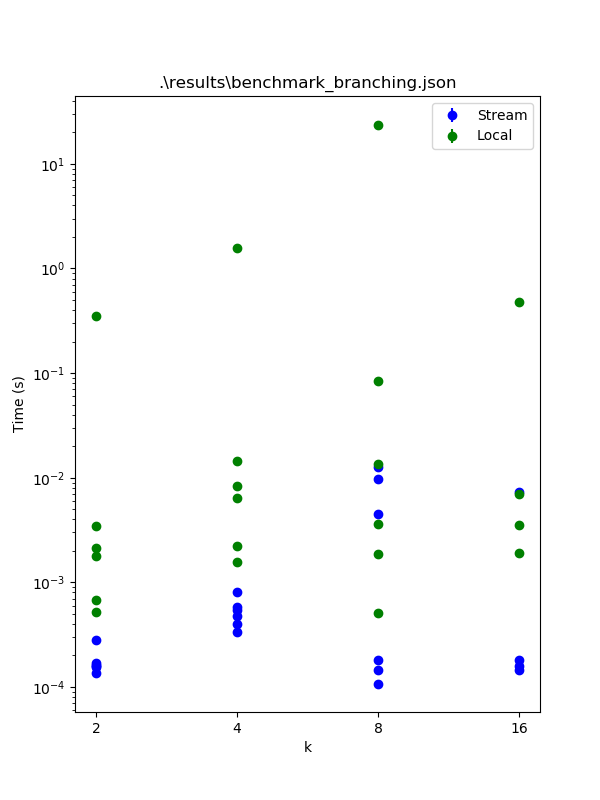
\includegraphics[width=\textwidth]{benchmark_time_branching.png}
    \caption{Runtimes of Branching}
    \label{fig:benchmark_time_branching}
\end{figure}

\subsection{Stream Implementation}

We built a graph streaming platform on top of Faust and Apache Kafka. Faust is
a Python stream processing library for use with Kafka. The platform consists of
one Faust instance serving as both the processor performing the algorithms and
a web server, and a second Faust instance serving as the source of the graph
stream. The web server serves a front end to clients shown in Figure
\ref{fig:stream_font_end}. From here users are able to create processing jobs
by selecting the algorithm, graph, and the \(k\) value from the top left box.
On submission of a job, the middle column shows the stream log of edges down
the middle column and, on completion, the right column displays a log of
results of each job. In early iterations of the system, logging every edge from
the incoming stream would freeze the entire site until the stream was finished.
Due to this, the stream log has been throttled in the number of updates it is
allowed to display per second and so should not be used as a true log as some
edges from the stream will be skipped. It has been left there as a visual cue
that an algorithm is running, plus it's interesting to see the data being
processed.

\begin{figure}[htb]
    \centering
    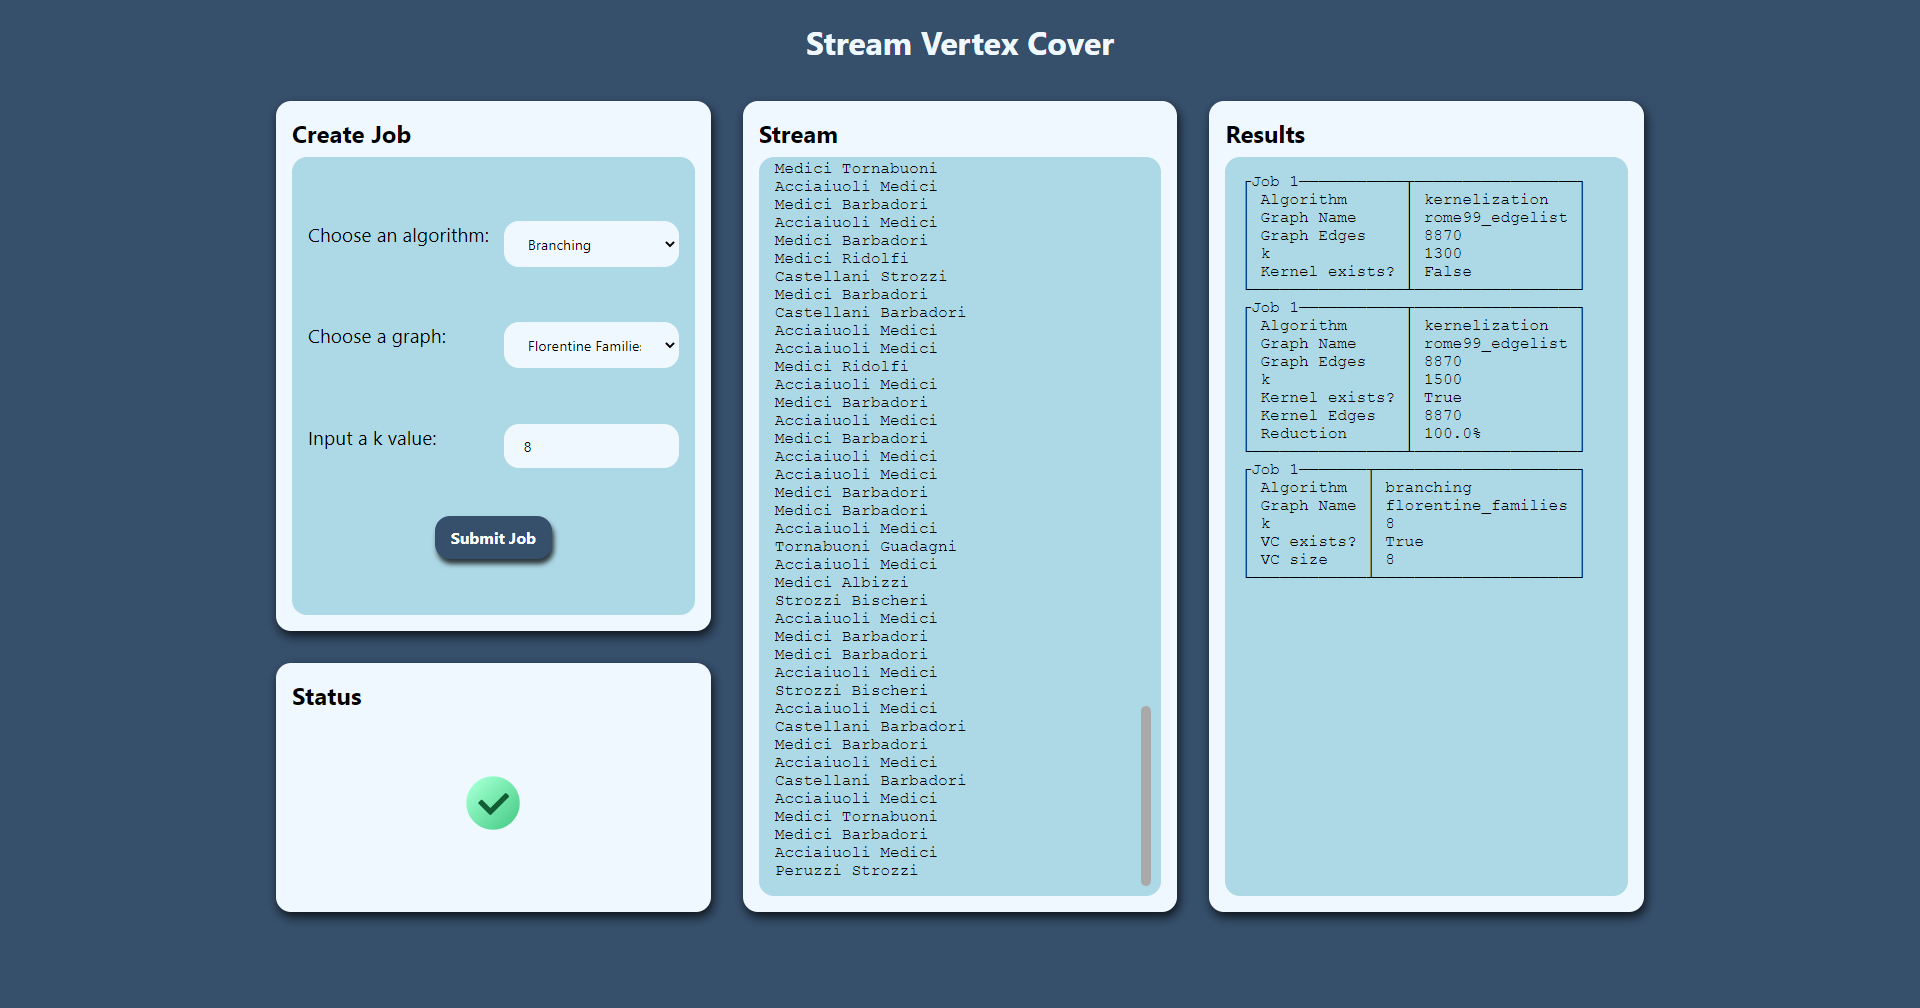
\includegraphics[width=\textwidth]{stream_new.png}
    \caption{Stream Implementation Front End}
    \label{fig:stream_font_end}
\end{figure}

The front end is built with HTML/CSS/JS and uses Server-Sent Events (SSE) for
the transmission of the stream and result logs. Originally, we had considered
using WebSockets, as the communication is bi-directional between the client and
server, but this introduced complexity in sorting through the different message
types (job submission/stream log/results log). It was deemed SSE was the better
option for the two logs and then a HTTP POST request could be used for the job
submission.

As this is a proof-of-concept, the second Faust instance was built purely for
development purposes. Once a graph is requested, it streams the edge list from
a file and then relays that into a Kafka topic. In the development environment,
it is run locally but, because it's built with Kafka, can be setup over a
network for a more typical production environment.

Kafka is platform agnostic in terms of the connections it allows since it only
facilitates the messaging between connections. This means that many different
data sources can be used, from databases to web crawlers.

\subsubsection{Control Flow}

We have three actors present in our system:

\begin{itemize}
    \item
          App (Client) - The browser client of the user
    \item
          App (Server) - The web server serving pages to the user and
          processing the algorithms
    \item
          Producer - The ``external'' server as the source of the stream of
          graph edges
\end{itemize}

For the kernelization algorithm the control flow is shown in Figure
\ref{fig:stream_kernelization}. The protocol used to communicate between each
actor is shown as a note covering between them.

\begin{figure}[H]
    \centering
    \begin{minipage}{.5\textwidth}
        \centering
        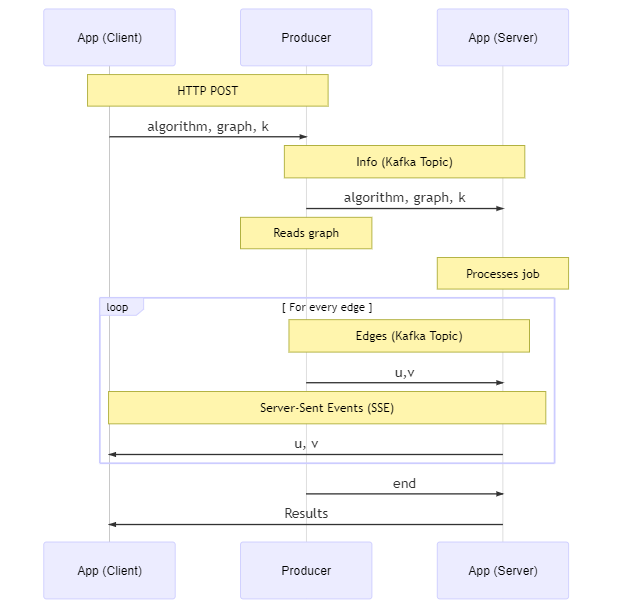
\includegraphics[width=\linewidth]{stream_kernelization.png}
        \captionof{figure}{Stream Kernelization Control Flow}
        \label{fig:stream_kernelization}
    \end{minipage}%
    \begin{minipage}{.5\textwidth}
        \centering
        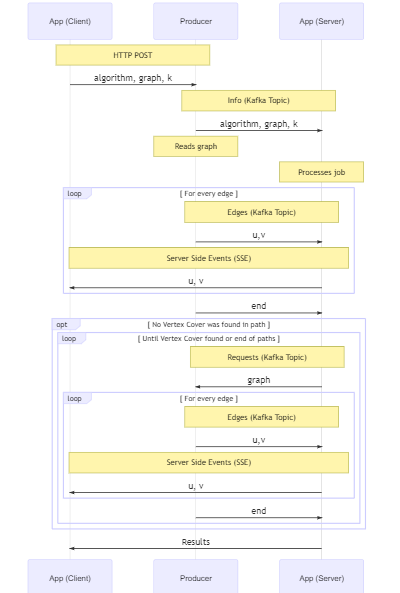
\includegraphics[width=\linewidth]{stream_branching.png}
        \captionof{figure}{Stream Branching Control Flow}
        \label{fig:stream_branching}
    \end{minipage}
\end{figure}

The branching algorithm requires a slightly different sequence of events due to
the fact that it is a multi-pass algorithm. The sequence is shown in Figure
\ref{fig:stream_branching}. As shown, some extra coordination is required for
the Server to request the graph to be streamed again by the Producer.
